\subsection{Introducci\'on} 

Para este ejercicio, se nos pide encontrar un algoritmo, que, dados $k$ caballos repartidos por un tablero de $n$ por $n$ casillas, encuentre cual es la casilla donde puedo reunir a todos los caballos en la menor cantidad de saltos.

Nuestra entrada ser\'a:

\begin{itemize}
\item Un entero \textbf{n} $\rightarrow$ Representar\'an el largo y el ancho del tablero.
\item Un entero \textbf{k} $\rightarrow$ Representar\'a el numero de caballos repartidos en el.
\item \textbf{k} filas donde, para cada fila se tiene:
\begin{itemize}
\item $f$ $c$ $\rightarrow$ Representar\'an la fila y la columna de cada caballo.
\end{itemize}
\end{itemize}

A esto nuestro algoritmo deve devolver:
\begin{itemize}
\item Un entero \textbf{f c} $\rightarrow$ Representar\'a la fila y columna a donde deven converger los caballos.
\item Un entero \textbf{m} $\rightarrow$ Representar\'a el numero total de saltos que le costar\'a a todos los caballos llegar hasta ah\'i.
\end{itemize}

\subsection{Ejemplos y Soluciones}
Se procede ahora a realizar un ejemplo para ilustrar el problema.

Supongamos que tenemos un tablero de $4$ por $4$ con un caballo en la posici\'on $1$,$1$ y otro en la posici\'on $4$,$4$.

La entrada del problema luego ser\'ia:

\begin{itemize}
\item $4$ $2$ 
\item $1$ $1$
\item $4$ $4$
\end{itemize}

Para este caso es posible encontrar una soluci\'on a mano, por ejemplo, es facil ver que en dos movimientos es posible hacer converger a amobos caballos.

En caso de querer asegurarnos de ello, podr\'iamos hacer lo siguiente. Dibujamos en un papel dos matrices de $n$ por $n$. En la primera matriz, vamos a poner cual es la cantidad minima de saltos que el primer caballo realiza para saltar a cada una de las casillas del tablero. 

Para ello primero anotamos en la matriz con costo $0$ la posicion donde se encuentra el primer caballo. Ahora, saltamos desde esta pocicion a todas las posibles pociciones validas del tablero. Todas estas tendran costo $1$.

Ahora, desde todas las pociciones de costo $1$ saltamos a todas las pociciones validas del tablero que podamos. Estas van a tener costo $2$. Si seguimos realizando este procedimiento, demostraremos que obtendremos la cantidad minima de saltos que el primer caballo realiza para saltar a cada una de las casillas del tablero, que era lo que buscabamos.

Realizamos lo mismo con el segundo caballo, marcamos la casilla donde se encuentra parado con costo $0$ y empezamos a saltar a las casillas validas.

Ahora sumamos ambas matrices, y lo que obtenemos es una matriz con los costos minimos de que todos los caballos salten a cada una de las posiciones del tablero.

Buscando los minimos en esta matriz, obtenemos lo que quer\'iamos! (me siento re paenza escribiendo estas cosas)




$$\textbf{SE PODRIAN AGREGAR DIBUJUTOS CON LAS MATRICES PARA QUE QUEDE CLARO}$$


Luego, algunas soluciones que el algoritmo podr\'ia devolver en este caso son:

\begin{itemize}
\item $1$ $1$ $2$ 
\item $2$ $3$ $2$
\item $4$ $4$ $2$ 
\end{itemize}

\subsection{Desarrollo}
La idea general del algoritmo es sencilla, para cada caballo, confeccionamos una matriz con el costo minimo de saltar a cada uno de los casilleros de la matriz. Luego sumando estas $k$ matrices, obtenemos el costo minimo de que cada caballo salte a cada uno de los casilleros.

Para asegurarnos de que en cada paso estamos tomando efectivamente la menor cantidad de saltos para que un caballo llegue a un casillero de la matriz, podemos pensar a la misma como un grafo, en el cual dos nodos estan conectados si y solo si un caballo puede saltar de uno a otro de manera valida.

Luego solo basta realizar un BFS para obtener el costo minimo de que un caballo llegue a esa casilla.

Cabe destacar, que por una cuesti\'on de claridad, en la implementacion final, la idea de recorrer un grafo est\'a implicita, la misma solo nos ayuda a ver que tanto la complegidad como la correctitud son las adecuadas en el problema dado.

En la implementacion real, simplemente creamos $k$ matrices de enteros de $n$ por $n$. Luego para cada caballo, tomamos todos los nodos de distancia $j$, buscamos todos los nodos validos de distancia $j+1$ y los seteamos. Realizamos esto hasta que no quedan nodos no seteados y all\'i pasamos de caballo.

Mas formalmente:

\begin{algorithm}
\begin{algorithmic}[1]\parskip=1mm
\caption{void FuncionPrincipal()}

  \STATE{Generar $k$ matrices de $n$x$n$ todas seteadas en infinito}

  \STATE{Creo dos colas: colaDeProfundidadJ,colaDeProfundidadJmasUno }
  
  \STATE{Para cada caballo, tomo la casilla donde se encuentra y lo encolo en colaDeProfundidadJ}
  
  \STATE{~~~Creo un entero $j$ igual a 0}

  \STATE{~~~Mientras colaDeProfundidadJ no este vac\'ia.}

  \STATE{~~~~~Para toda casilla $\in$ colaDeProfundidadJ}

  \STATE{~~~~~~~~En la matriz correspondiente a este caballo, asigno j, como el valor del nodo}

  \STATE{~~~~~~~~Busco los vecinos, si estan seteados en infinito los encolo en colaDeProfundidadJmasUno}
  
  \STATE{~~~~~Sumo $1$ a $j$}

  \STATE{~~~~~Encolo los valores de colaDeProfundidadJmasUno en colaDeProfundidadJ}

  \STATE{~~~~~Vac\'io colaDeProfundidadJmasUno}

  \STATE{Sumo las $k$ matrices}

  \STATE{Busco el minimo}

  \STATE{imprimo el minimo}
 
 \end{algorithmic}
\end{algorithm}

\newpage
\subsection{Demostraci\'on De Correctitud}

Para demostrar la correctitud de este algoritmo, primero, demostramos que dada una matriz de $n$x$n$, $n\gdq 4$ desde cualquier casillero existe una sucesion de saltos para llegar a cualquier otro. 

Por induccion en $n$, siendo $n$ la cantidad de filas y de columnas.

Caso base:

$$\textbf{DIBUJITO}$$



Caso inductivo:
Luego, si existe el tablero de $n$x$n$ tal que de cualquier casillero podemos ir a cualquier casillero, quiero demostrar el tablero de $n+1$x$n+1$ tambien cumple.

Tomamos el casillero hubicado en la fila $n+1$ columna $1$ (que notamos $(n+1,1)$), y vemos que existe un salto al casillero ($n-1$,$2$), luego, existe una sucecion de saltos desde el casillero $(n+1,1)$ a cualquiera del tablero de $n$x$n$.

Para todos los casilleros en ($n+1$,$i$) con $i>1$, podemos saltar al casillero ($n-1$,$i-1$), y luego desde todos estos casilleros, tabmien podemos saltar dentro del tablero de $n$x$n$.

Ahora podemos ver que para la casilla ($1$,$n+1$), tambien existe el salto a ($2$,$n-1$), que hace que tambien cumpla.

De la misma manera, para los casilleros para ($i$,$n+1$) con $1< i \geq n+1$ existe el salto a la casilla ($i-1$,$n-1$).

Con lo cual concluimos que existe un salto desde cualquier casillero de la fila $n+1$ o columna $n+1$ podemos saltar a cualquier casillero del tablero de $n$x$n$, por lo tanto, por hipotesis inductiva, existe una sucecion de saltos para llegar a cualquier casillero del tablero, en particular, puedo ir desde cualquier casillero de la fila/columna $n+1$x$n+1$ a cualquier otro que pertenezca a la misma fila/columna.

A partir de un tablero de $nxn$ el modelado cada casillero representa un nodo, y dos nodos son adyacentes si y solo si existe un salto de caballo en el tablero.

Por la demostracion anterior, sabemoos que desde cualquier casillero existe una sucecion de saltos para llegar a cualquier otro, traducido a nuestro modelo de grafo, quiere decir que este es conexo.

Como el grafo es conexo y finito, realizando un bfs para cada caballo, podemos obtener la cantidad minima de saltos desde la pocicion en la que se encuentra el caballo hasta todas las otras del tablero.

Por lo tanto, sumando cuantos saltos debe realizar cada caballo a cada casillero, obtengo el minimo de saltos que tienen que dar todos los caballos para llegar a cualquier casillero.

Para cada casillero, sumanos los saltos de cada caballo y nos quedamos con el que tenga suma minima.

\subsection{Complejidad}
Para cada caballo, encolamos una sola vez cada nodo y posteriormente lo procesamos.

Entonces la complegidad es la cantidad de caballos ($k$) por la cantidad de nodos ($n^2$).

En otras palabras la complegidad es $O(kn^2)$.

\subsection{Experimentacion}
Para testear la performance de nuestro algoritmo se cre\'o un generador de entradas que fabricar\'a instancias random del problema.

Para la primera experimentaci\'on se deja el tablero fijo, y se var\'ia el numero de caballos. Para este testeo, se tom\'o $n = 100$ y se hizo variar el numero de caballos entre 50 y 1500, cada uno posicionado de manera aleatoria en una casilla, y se tomaron $50$ muestras de cada uno.

Los resultados obtenidos se muestran en el siguiente grafico.

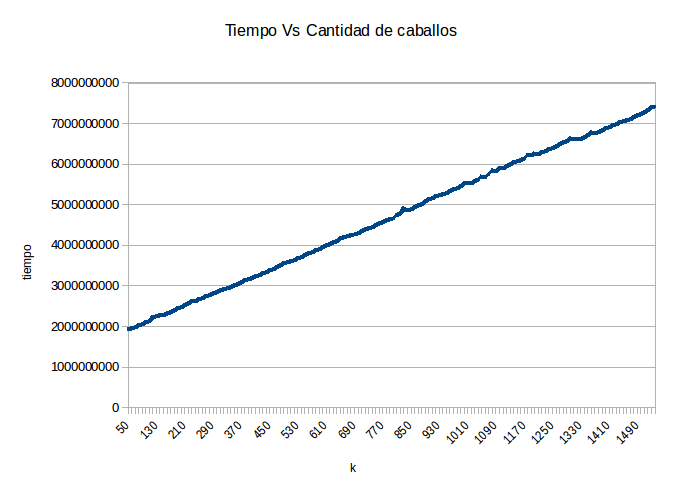
\includegraphics[scale=0.7]{Ej2/testing_k.png}

Puede verse claramente que el algoritmo se comporta de manera lineal con respecto a la cantidad de caballos